In the previous chapter, we have seen how the many-body problem can be decoupled into an electronic problem given by Eq.\,\eqref{eq:Hsolution1}, which can be solved in the framework of DFT, and a nuclear problem given by Eq.\,\eqref{eq:chi2} that describes the dynamical properties of the nuclei. This was achieved by means of the Born-Oppenheimer approximation where electron-nucleus interactions beyond a parametric dependence on each other is neglected~\cite{BornOppenheimer}.

We will now introduce two approximations to progress in the description of the nuclear dynamics. First, the \emph{harmonic approximation} in which the nuclear Schr\"odinger equation is solved for an approximated potential. Second, we treat the nuclei as particles, but on the full, non-truncated Born-Oppenheimer potential. This will lead to the formulation of \emph{ab initio molecular dynamics} (aiMD). As no electron will appear anymore, $N \equiv N_{\rm Nuc}$ will henceforth denote the number of nuclei in the system of interest, and we denote the Born-Oppenheimer potential simply as \emph{the} potential, $\mathcal V ({\bf R})$.

We begin by recalling the Schr\"odinger equation for the nuclear wavefunctions $\chi_s ({\bf R})$ initially defined in Eq.\,\eqref{eq:chi2},
\begin{align}
  \left( T^{\rm Nuc} + \mathcal V ({\bf R}) - E \right) \chi ({\bf R})
  = 0~,
  \label{eq:BOSE}
\end{align}
where
\begin{align}
  T^{\rm Nuc}
    = \sum_I \frac{- \hbar^2}{2 M_I} \frac{\partial^2}{\partial {\bf R}_I^2}~,
  \label{eq:Tnuc2}
\end{align}
is the nuclear kinetic-energy operator as before.

\subsection{Harmonic Approximation}
The Born-Oppenheimer potential $\mathcal V ({\bf R})$ appearing in Eq.\,\eqref{eq:BOSE} is an ordinary function of the $3 N_{\rm Nuc}$ coordinates ${\bf R} = ({\bf R}_1, \ldots, {\bf R}_{N_{\rm Nuc}})$ and therefore can be expanded as a Taylor series in displacements ${\bf U} \equiv \Delta {\bf R}$ about a given configuration ${\bf R}^0$,~i.\,e.,
\begin{align}
\begin{split}
  \mathcal V ({\bf R} = {\bf R}^0 + {\bf U})
    = \mathcal V ({\bf R}^0)
    &+ \sum_{I, \alpha} 
      \left. \frac{\partial \mathcal V({\bf R})}{\partial R^\alpha_I} 
      \right\vert_{{\bf R}^0}
    \,U^\alpha_I
    \\
    &
    + \frac{1}{2}
    \sum_{\substack{I, J \\ \alpha, \beta}}
    \left.\frac{\partial^{2} \mathcal{V}(\mathbf{R})}{\partial R_{I}^{\alpha} \partial R_{J}^{\beta}}\right|_{\mathbf{R}^{0}}
    \, U_I^\alpha U_J^\beta
    \\
    &+\frac{1}{3!}\cdots ~,
\end{split}
\end{align}
where the expansion coefficients are called \emph{force constants}. In particular, we have
\begin{align}
  % \Phi_{\alpha, \beta}^{I, J}
  \Phi_{I \alpha, J \beta}
  \equiv \left.\frac{\partial^{2} \mathcal{V}(\mathbf{R})}{\partial R_{I}^{\alpha} \partial R_{J}^{\beta}}\right|_{\mathbf{R}^{0}}~,
  \label{eq:FC2}
\end{align}
i.\,e.,~the \emph{harmonic force constants}. The harmonic approximation is typically used to assess dynamical properties of a system in some confined phase-space region close a (local) minimum of the potential-energy surface. It is therefore customary to start the investigation from the ground state of the system,~i.\,e.,~a local minimum configuration ${\bf R}^0$ characterized by
\begin{align}
	\left. \frac{\partial V({\bf R})}{\partial R^\alpha_I} 
	\right\vert_{{\bf R}^0} 
		&~=~ 0 \quad\text{for all}\quad (I, \alpha),~\text{and} \\
	\sum_{\substack{I, J \\ \alpha, \beta}}
	% \Phi_{\alpha, \beta}^{I, J}
	\Phi_{I \alpha, J \beta}
	\, U_I^\alpha U_J^\beta
		&~>~ 0 \quad\text{for all possible}\quad \set{{\bf U}_I}~.
	\label{eq:ha.positive}
\end{align}
The condition in Eq.\,\eqref{eq:ha.positive} is fulfilled if the harmonic force constants $\Phi_{\alpha, \beta}^{I, J}$ are positive-definite.

We progress by defining \emph{mass-reduced coordinates} for the displacements
\begin{align}
	{\bf u}_I 
		&\equiv \sqrt{M_I} {\bf U}_I~, 
		\label{eq:uI} \\
	{\bf p}_I 
		&\equiv -\im \hbar \frac{\partial}{\partial {\bf u}_I}~,
		\label{eq:pI} \\
	% D_{\alpha, \beta}^{I, J}
	D_{I \alpha, J \beta}
		&\equiv \frac{1}{\sqrt{M_I M_J}} 
		%\Phi_{\alpha, \beta}^{I, J}
		\Phi_{I \alpha, J \beta}~,
		\label{eq:D}
\end{align}
where Eq.\,\eqref{eq:D} defines the \emph{dynamical matrix} $\rm D$.
Using these coordinates, the Hamiltonian assumes the form
\begin{align}
	\begin{split}
		\mathcal{H}({\bf p}, {\bf u})
			&= T^{\rm Nuc} ({\bf p}) + \mathcal{V}^{(2)} ({\bf u})\\
			&= \halb \sum_I {\bf p}_I^2 + 
				\halb \sum_{\substack{I, J \\ \alpha, \beta}}
					D_{I \alpha, J \beta}
					\, u_I^\alpha u_J^\beta~.
	\end{split}
	\label{eq:ha.H1}
\end{align}
As required earlier, the dynamical matrix $\rm D$ is a positive definite matrix. Furthermore, we see from Eq.\,\eqref{eq:FC2} that
\begin{align}
	D_{I \alpha, J \beta} = D_{J \beta, I \alpha}~,
	\label{eq:D.symmetric}
\end{align}
i.\,e.,~$\rm D$ is a symmetric matrix in the $3N$ coordinates $(I, \alpha)$. The eigenvalues of $\rm D$ will therefore be real and positive, and the eigenvectors will be real and orthogonal. We denote the eigenvalues as $\omega_s^2$ and the normalized eigenvectors as ${\bf e}_s$, where $s$ is the \emph{mode} label. $\omega_s$ will have the unit of a frequency and  will be called \emph{eigenfrequency} in the following. The dynamical matrix elements can be rewritten in therms of the eigenvectors and eigenvalues as
\begin{subequations}
\begin{align}
	\sum_{J \beta}
		D_{I \alpha, J \beta} \, e_{s, J \beta} 
			&= \omega^2_s \, e_{s, I \alpha}~,~\text{or} 
			\label{eq:sum_D_IJ} \\
		D_{I \alpha, J \beta}
			&= \sum_s \omega^2_s \, e_{s, I \alpha} e_{s, J \beta}~.
			\label{eq:D_IJs}
\end{align}
\end{subequations}
Since the eigenvectors fulfill
\begin{align}
	\sum_{I \alpha} e_{s, I \alpha} e_{s', I \alpha} = \delta_{s s'}
	\quad \text{and} \quad
	\sum_{s} e_{s, I \alpha} e_{s, J \beta} = \delta_{IJ} \delta_{\alpha \beta}~,
\end{align}
we can rewrite the Hamiltonian in Eq.\,\eqref{eq:ha.H1} by using the dynamical matrix elements as defined in Eq.\,\eqref{eq:D_IJs}, so that
\begin{align}
	\mathcal{H}( {\bf p},  {\bf u})
		&= \halb \sum_s p_s^2 + 
		\halb \sum_{s} \omega_s^2	\, u_s^2~.
\label{eq:ha.H2}
\end{align}
Here, we implicitly defined the \emph{normal coordinates} $u_s$ and their conjugate momenta $p_s$,~i.\,e.,
\begin{align}
	u_s
		&= \sum_{I \alpha} e_{s, I \alpha} \, u_{I \alpha}~,
		\label{eq:u_s} \\
	p_s
		&= -\im \hbar \frac{\partial}{\partial u_s}~.
		\label{eq:p_s}
\end{align}
The Hamiltonian expressed in terms of the normal coordinates, Eq.\,\eqref{eq:ha.H2}, contains no cross-terms between different modes $s$ and $s'$. Rewritten in terms of this Hamiltonian, the wave equation \eqref{eq:BOSE} reads
\begin{align}
	\left\{
		\halb \sum_s p_s^2 + \halb \sum_{s} \omega_s^2	\, u_s^2 - E~.
	\right\} \chi ({\bf u})
	= 0
	\label{eq:ha.SE.2}
\end{align}
Since the Hamiltonian is a sum of terms, each depending on one coordinate only, the total nuclear wavefuntion $\chi$ can be separated into a product of wavefunctions for each mode,
\begin{align}
	\chi({\bf u}) = \prod_{s} \chi_s (u_s)~.
	\label{eq:ha.chi}
\end{align}
We end up with a set of $3N$ uncoupled equations, one for each mode $s$:
\begin{align}
	\left\{	\halb \left( p_s^2 + \omega_s u_s^2 \right)	- E_s	\right\} \chi_s (u_s)
		= 0~,
	\label{eq:ha.SE.single}
\end{align}
where the total energy of the nuclei is the sum of each mode contribution $E = \sum_s E_s$. Equation \eqref{eq:ha.SE.single} is the familiar equation for a harmonic oscillator of frequency $\omega_s$~\cite{Dirac1981}. Permissible solutions are labeled by the integer $n_s \in \mathds N_0$ and the eigenvalue $E_s$ depends on $n_s$ via
\begin{align}
	E_s(n_s) = \hbar \omega_s \left( n_s + \halb \right)~.
	\label{eq:E_s}
\end{align}
The state of the entire system is therefore specified by the $3N$ quantum numbers ${\bf n} = (n_1, \ldots, n_{3N})$, and the total energy of the system is
\begin{align}
	E ({\bf n}) = \sum_s \hbar \omega_s \left( n_s + \halb \right)~.
\end{align}
The thermodynamic properties of such a system of harmonic oscillators follow from this spectrum in straighforward fashion~\cite{BornHuang}.

This derivation is generally valid for a system of $N$ particles described by a potential-energy surface of which a (local) minimum ${\bf R}^0$, and the matrix of second derivatives at this configuration, $\Phi^{IJ}$, is known.

\subsubsection{Periodic Systems}
As already mentioned in Sec.~\ref{sec:theory.periodic.1}, the crystalline state is characterized by a periodic long-range order described the Bravais vectors ${\bf L} = L^i {\bf a}_i$, where $\set{{\bf a}_i}$ is the crystal basis and $L^i \in \mathds Z$.
We define this symmetry as follows:
Let ${\bf R}^0 = \set{{\bf R}_I^0}$ be the configuration of atoms in the local minimum of interest, and let ${\bf R}^{0 \prime} = \set{{\bf R}^{0 \prime}_{I}}$ denote the configuration obtained by moving all atoms by a Bravais vector ${\bf L}$,
\begin{align}
	{\bf R}^{0 \prime}_{I} = {\bf R}^0_{I} + {\bf L}~.
	\label{eq:RI'}
\end{align}
As a prerequisite for $\mathcal V ({\bf R})$ to be translationally invariant, we require that ${\bf R}^{0 \prime} = \set{{\bf R}^{0 \prime}_{I}}$ is a minimum configuration of the potential as well, \emph{and} there is a bijective permutation map $P_{\bf L}$ between the atomic positions ${\bf R}^{0 \prime}_{I}$ and ${\bf R}^{0}_{I'}$ which fulfills
\begin{align}
	P_{\bf L} : I \to I' \quad\text{such that}\quad
	{\bf R}^{0 \prime}_{I}
		= {\bf R}^{0}_{I'}~,
	\label{eq:translation.permutation}
\end{align}
i.\,e.,~the configurations ${\bf R}^{0 \prime}_{I}$ and ${\bf R}^{0}_{I}$ are indistinguishable.\,\footnote{This requirement is obviously not fulfilled for molecules, where rigidly shifting all atoms can by no means induce a permutation map between atoms.} 
The final requirement for translational invariance of the potential is that the potential energy for \emph{any} configuration differing by a Bravais vector is unchanged:
\begin{align}
%	{\bf R}^{0 \prime}
%	= \set{{\bf R}_{I'}^0 }
%	&= {\bf R}^0 = \set{{\bf R}_{I}^0 }~,
%	\quad\text{and}
%	\label{eq:inv.R0} \\
	\mathcal{V} \left( {\bf R}' = \set{{\bf R}_{I} + {\bf L}} \right)
	&= \mathcal{V}({\bf R} = \set{{\bf R}_{I}} ) 
	\quad\text{for all}\quad {\bf L} = L^i {\bf a}_i~.
	\label{eq:inv.V}
\end{align}
This effectively corresponds to a permutation of the displacements of the atoms, $U_I \to U_{I'}$ according to $P_{\bf L}$. Figure\,\ref{fig:translation.permutation} shows a one-dimensional depiction of the relation between discrete translation by Bravais vectors and the permutation map.
\begin{figure}[h]
	\centering
	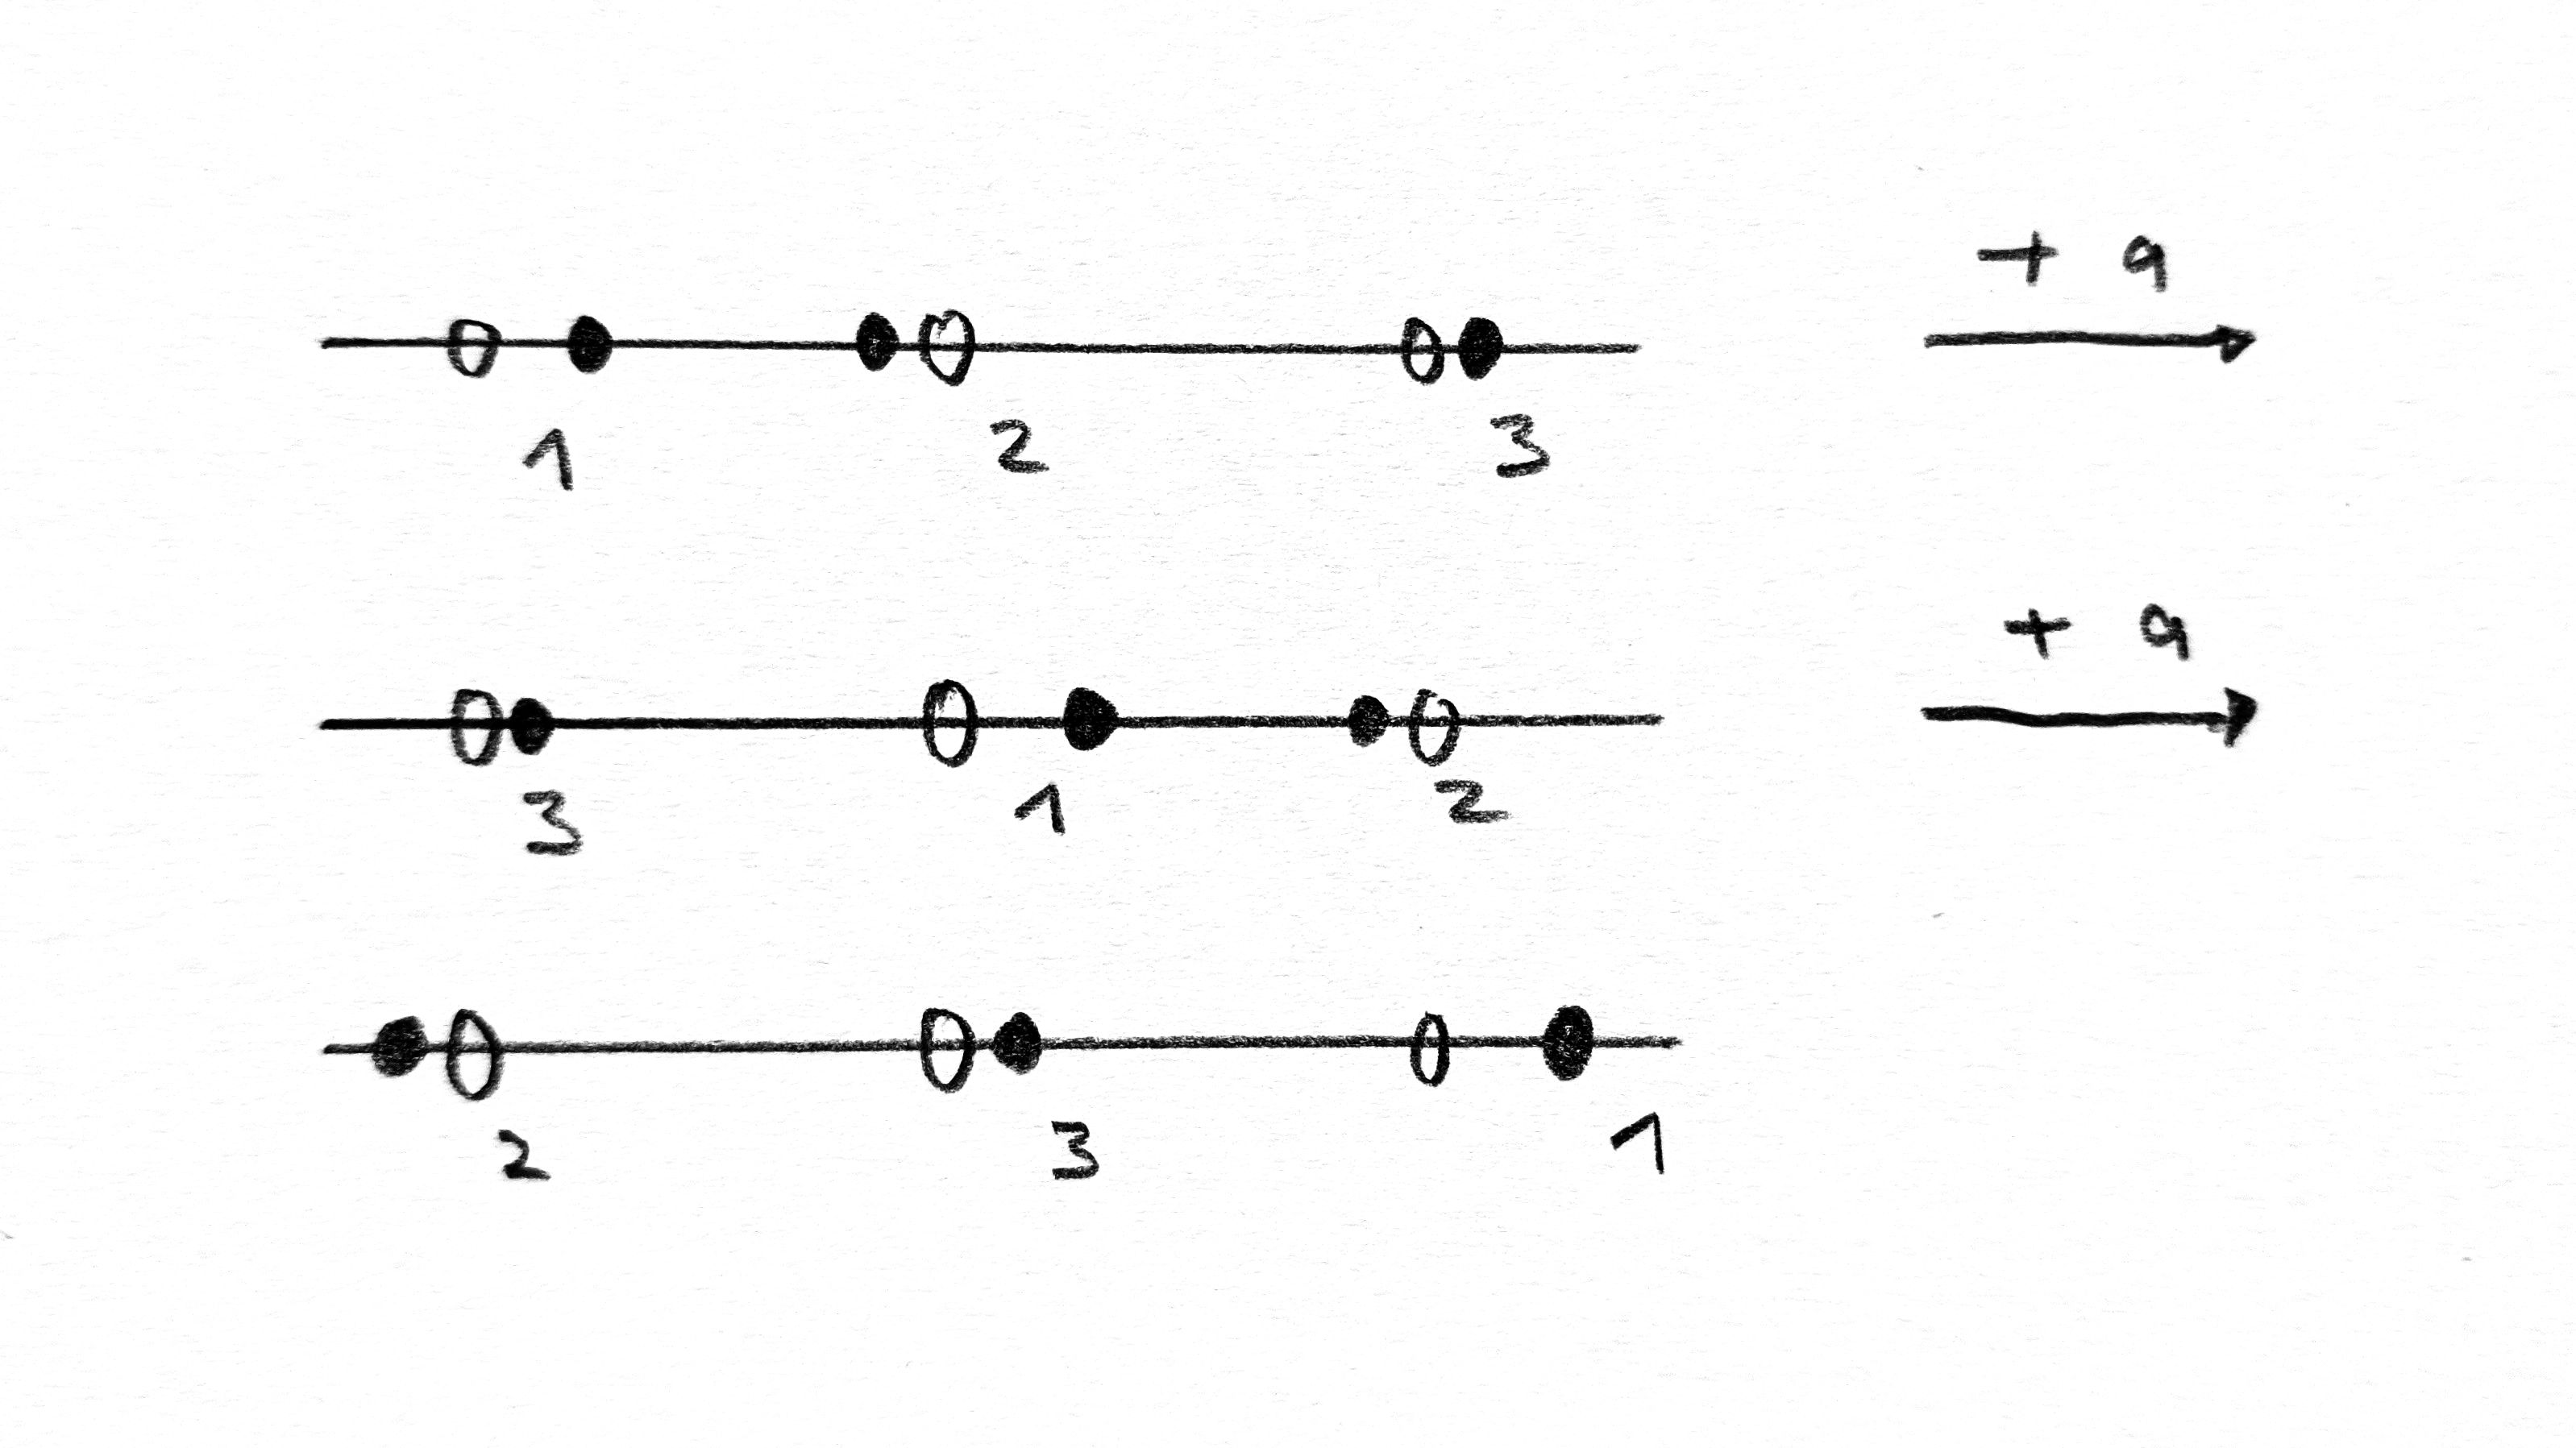
\includegraphics[width=.68\textwidth]{./sketches/permutation1.jpg}
	\caption{A linear chain with three atoms (bullets) displaced from their equilibrium position (open circels). With periodic boundary conditions, the consecutive translation by a lattice vector $a$ induces a permutation of the atoms,~i.\,e.,~$(1, 2 , 3) \to (3, 1, 2) \to (2, 3, 1)$.}
	\label{fig:translation.permutation}
\end{figure}

We can draw several important conclusions from Eq.\,\eqref{eq:translation.permutation} and \eqref{eq:inv.V}. First, the existence of the map $P_{\bf L}$ enables us to write every atomic coordinate ${\bf R}_I$ as
\begin{align}
	{\bf R}_I \equiv {\bf R}_{i {\bf L}} 
		= {\bf R}^0_i + {\bf U}_{i {\bf L}} + {\bf L}~,
	\label{eq:R_iL}
\end{align}
where ${\bf R}^0_i$ labels the position of an equivalent reference atom in the unit cell, ${\bf U}_{i {\bf L}}$ is the displacement of the atom from its equilibrium position, and $\bf L$ is a Bravais vector as before.
We can therefore split the index $I$ into a tuple $I = (i, {\bf L})$,~i.\,e.,~uni cell and lattice point labels.

Second, the harmonic force constants $\Phi_{I \alpha, J \beta}$ can be written as $\Phi_{i {\bf L} \alpha, j {\bf K} \beta}$~, where $\bf L$ and $\b K$ are the Bravais vectors belonging to $I$ and $J$, respectively. From the translational invariance of the potential, Eq.\,\eqref{eq:inv.V}, we see that the force constants have to fulfill
\begin{align}
	\Phi_{i {\bf L} + \b M \alpha, j {\bf K} + \b M \beta} 
		= \Phi_{i {\bf L} \alpha, j {\bf K} \beta}~,
	\label{eq:fc.sym.1}
\end{align}
where $\b M$ again denotes an arbitrary Bravais vector. Using this translational invariance, we can Fourier transform the dynamical matrix defined in Eq.\,\eqref{eq:D},
\begin{align}
	{\rm D}_{i \alpha, j \beta} (\b q) 
		= \sum_{\b L} {\rm e}^{- \im \b q \cdot \b L} {\rm D}_{i \b 0 \alpha, j \b L \beta}
	\label{eq:D(q)}
\end{align}
where we restrict the values of $\b q$ to reside in the first Brillouin zone, thereby transforming the $3N \times 3N$ matrix ${\rm D}_{IJ}$ to one $3n \times 3n$ matrix ${\rm D}_{ij} (\bf q)$ for each~$\b q$, where $n$ is the number of atoms in the primitive unit cell.

\subsubsection{Cyclic Boundary Conditions and Supercell Approximation}
In the previous section, we did not specify the system beyond requiring periodic boundary conditions, and implicitly assumed an infinite crystal in the limit $N \to \infty$ without boundaries. In practice we introduce Born-von Karman cyclic boundary conditions~\cite{born2013atomtheorie}, as already done in Sec.\,\ref{sec:theory.periodic.1} for the description of electronic states, but reintroduce them here in a slightly more general fashion.

We define the boundary conditions for the nuclear problem such that
\begin{align}
	\b R_I + S^i \b A_i = \b R_I \quad\text{for}\quad S^i \in \mathds{Z}~,
	\label{eq:sc.1}
\end{align}
where each ${\bf A}_i$ is a linear combination of the primitive basis vectors $\set{{\bf a}_i}$,
\begin{align}
{\bf A}_i = {\rm M}_{ij}^{\rm sc} {\bf a}_j\quad\text{with } {\rm M}_{ij}^{\rm sc} \in \mathds Z~,
\end{align}
and $\rm M^{\rm sc}$ is a non-singular matrix with integer elements. The space spanned by the $\set{{\bf A}_i}$ is parallelepiped of volume $V_{\rm sc} = N_{\rm sc} \, {\bf a}_1 \cdot ({\bf a}_2 \times {\bf a}_3)$, where $N_{\rm sc} = \det {\rm M}^{\rm S}$ is the number of unit cells that fit into the enlarged cell, and $V_{\rm uc} = {\bf a}_1 \cdot ({\bf a}_2 \times {\bf a}_3)$ is the unit cell volume. This cell is therefore called \emph{supercell}, and the matrix ${\rm M}^{\rm S}$ is denoted as the \emph{supercell matrix}. The vectors $\b S = S^i \b A_i$ are the equivalent of the Bravais vectors $\b L$ in a superlattice described by $\set{ \b A_i }$ instead of $\set{ \b a_i}$.
The ideal, infinite crystal is obtained in the limit $N_{\rm sc} \rightarrow \infty$.
From Eq.\,\eqref{eq:sc.1} we see that the force constants need to fulfill
\begin{align}
	\Phi_{i {\bf L} \alpha, j {\bf K} + \b S \beta} 
		= \Phi_{i {\bf L} \alpha, j {\bf K} \beta} \quad\text{for all}\quad \b S = S^i \b A_i~,
	\label{eq:fc.sym.2}
\end{align}
so that the dynamical matrix in Eq.\,\eqref{eq:D(q)} can be written as a sum over lattice points that are contained in the supercell only,
\begin{align}
	{\rm D}_{i \alpha, j \beta} (\b q) 
%		&= \sum_{\b L \in V_{\rm sc}} 
%			\left( 
%				{\rm e}^{- \im \b q \cdot \b L} {\rm D}_{i \b 0 \alpha, j \b L \beta}
%			+ \sum_{\b S \neq \b 0} {\rm e}^{- \im \b q \cdot (\b L + \b S)} {\rm D}_{i \b 0 \alpha, j \b L \beta}
%			\right)~
%	\label{eq:D^S(q).1} \\
	&= %\frac{N}{N_{\rm sc}} 
	\sum_{\b L \in V_{\rm sc}} {\rm e}^{- \im \b q \cdot \b L} {\rm D}_{i \b 0 \alpha, j \b L \beta}~,
	\label{eq:D^S(q).2}
\end{align}
for $\b q$ that fulfill
\begin{align}
	{\bf q} \cdot {\bf A}_i	= 2 \pi m_i \quad\text{with}\quad m_i \in \mathds Z~.
	\label{eq:q.commensurate}
\end{align}
% the summands in the second sum of Eq.\,\eqref{eq:D^S(q).1} interfere constructively and yield a factor $\sum_{\b S}' = N / N_{\rm sc} - 1$. For all other $\b q$, the entire summand becomes negligible in the limit $N \to \infty$.
The $\b q$ that fulfill Eq.\,\eqref{eq:q.commensurate} are called \emph{commensurate} $\b q$-points, as they represent wave numbers that fit into the supercell.
In total there are $N_{\rm sc}$ permissible values of $\bf q$ labelled by ${\bf m} = (m_1, m_2, m_3)$ that can be expressed in terms of the lattice vectors of the reciprocal supercell,
\begin{align}
{\bf B}^i 
= 2 \pi \varepsilon^{ijk} \frac{{\bf A}_j \times {\bf A}_k}{{\bf A}_1 \cdot ({\bf A}_2 \times {\bf A}_3)} ~,
%\label{eq:dft.Bloch.bi}
\end{align}
where $\varepsilon^{ijk}$ denotes the Levi-Civita symbol enforcing the correct ordering of $ijk$. The complete set of $\bf q$-values is
\begin{align}
{\bf q}_{\bf m} 
= \sum_{i=1}^3 m_i {\bf B}^i~,
%\label{eq:dft.Bloch.k_m}
\end{align}
with $m_i \in \mathds Z$ such that $\b q_{\bf m}$ is an element of the first Brillouin zone of the direct lattice.

%As we will be interested in the eigenvalues and eigenvectors of the dynamical matrices $\rm D ({\b q})$, the prefactor $N/N_{\rm sc}$ can be neglected in the following.

\REM{for $\b q = \b q_{\b m}$ D is exact up to boundary effects (?!), nevertheless one can interpolate -> Fourier interpolation}
\REM{Alternative: Use effective cutoff of $\Phi$}
\REM{Effective cutoff -> effect on spectrum, Maradudin, Ledermann}

% Equation~\eqref{eq:D^S(q).2} will in general not be hermitian in $(i \alpha, j \beta)$

For each $\b q$, ${\rm D} (\b q)$ is a hermitian $3n \times 3n$ matrix in the indices $(i \alpha, j \beta)$ and will therefore yield $3n$ real eigenvalues and $3n$ complex, orthogonal eigenvectors, which denote in accordance with Eq.\,\eqref{eq:sum_D_IJ}
\begin{align}
	\sum_{j \beta} {\rm D}_{i \alpha, j \beta} (\b q) e_{j \beta} (\b q , b)
		= \omega^2 \, (\b q, b) e_{i \alpha} (\b q , b)~,
	\label{eq:D_ij(q)w}
\end{align}
where the \emph{band index} $b$ is used to discern the $3n$ \emph{branches} at each $\b q$. Using the combined index $s = (\b q, b)$, the notation becomes similar to the non-periodic case with $3N_{\rm sc} N_{\rm uc}$ degrees of freedom, only that the eigenvectors $\b e_{s = (\b q, n)}$ can be complex valued instead of strictly real.
\REM{This is Born conventions. Togo and Parlinski use extra phase factor ${\rm e}^{\im \b q \cdot (\b R_i^0 - \b R_j^0)}$ that alters the eigenvectors but not the frequencies.}

\subsubsection{Ledermann's Theorem}

\subsubsection{Finite Differences}

\subsection{Harmonic Sampling}

\subsection{Molecular Dynamics}
The classical limit of the nuclear Schr\"odinger equation~\eqref{eq:BOSE} is usually performed by writing the nuclear wavefunction $\chi_s ({\bf R}, t)$ in terms of a real amplitude $A_s({\bf R}, t)$ and a \emph{classical action function} $S_s({\bf R}, t)$~\cite{Dirac1981,Landau2013,Marx2009}
\begin{align}
	\chi_s({\bf R}, t) = A_s({\bf R}, t) \, {\rm e}^{\frac{\im}{\hbar} S_s({\bf R}, t)}~.
	\label{eq:class.1}
\end{align}
The Schr\"odinger equation then yields a set of differential equations for $A_s$ and $S_s$ that, in the limit $\hbar \to 0$, go over to a \emph{Hamilton-Jacobi} equation for $S_s$,~i.\,e.,~
\begin{align}
  \frac{\partial S_s}{\partial t} + \mathcal H \left({\bf R}, {\bf P}\right)
  = 0~,
  \label{eq:HamiltonJacobi}
\end{align}
where ${\bf P} = ({\bf P}_1, \ldots) \equiv ({\bf \nabla}_1 S_s, \ldots)$ denotes the conjugate momenta and $\mathcal H$ is the \emph{classical} Hamilton function corresponding the to the operator in Eq.\,\eqref{eq:BOSE}, from which the equations of motion for the nuclei can be obtained:
\begin{align}
  \dot{{\bf P}}_I 
    = -\frac{\partial \mathcal H}{\partial {\bf R}_I}
    \quad\implies\quad M_I \ddot{\bf R}_I
    = -\frac{\partial \mathcal V}{\partial {\bf R}_I}~.
    % \equiv - {\bf F}_I~.
\end{align}
The negative gradient of the Born-Oppenheimer potential, 
$-\partial \mathcal V / \partial {\bf R}_I$ is the force ${\bf F}_I$ acting on atom $I$ which can be obtained via the Hellmann-Feynmann theorem,~cf.~Sec.\,\ref{sec:HellmannFeynman}.

An alternative viewpoint that is more instructive can be taken by invoking the \emph{Ehrenfest theorem}~\cite{Ehrenfest1927,Basdevant2007}. The statement is that
\begin{align}
  \frac{\d}{\d t} \left\langle {\bf P}_I \right\rangle_{\chi_s}
    = \left\langle
      - \frac{\partial \mathcal{V}}{\partial {\bf R}_I}
    \right\rangle_{\chi_s}~,
  \label{eq:ehrenfest.de1}
\end{align}
where $\langle \cdot \rangle_{\chi_s}$ denotes an expectation value taken with respect to the state $\chi_s$. This expression differs only slightly from the classical counterpart, which would read
\begin{align}
\frac{\d}{\d t} \left\langle {\bf P}_I \right\rangle
= \left.
- \frac{\partial \mathcal{V}}{\partial {\bf R}_I}
\right\vert_{{\bf R} = \langle {\bf R} \rangle}~.
\label{eq:ehrenfest.de2}
\end{align}
The difference comes from the fact that, in general,
\begin{align}
  \delta f  \equiv 
  f \bm ( \langle x \rangle \bm{)} 
  - 
  \bm{\langle} f (x) \bm{\rangle}
  \neq 0
  ~,
  \label{eq:ehrenfest.delta1}
\end{align}
where $x = {\bf R}_I$ denotes the space coordinate for notional simplicity, $f$ is some function of the observable $x$, and $\delta f$ measures the difference between the classical and the quantum expectation value. Ehrenfest's argument is that this difference becomes negligible when the state is sufficiently peaked around some value $x_0$. Expanding $f$ around the expectation value of $x$, $x_0 \equiv \langle x \rangle$, we have
\begin{align}
  f(x) = f \bm ( \langle x \rangle \bm{)}  
    + (x - \langle x \rangle) \, f' \bm ( \langle x \rangle \bm{)}
    + \frac{1}{2} (x - \langle x \rangle)^2 \, f'' \bm ( \langle x \rangle \bm{)}
    + \cdots~.
  \label{eq:ehrenfest.f2}
\end{align}
It follows that the $f'$ term vanishes when the expectation value is taken, and
\begin{align}
\langle f(x) \rangle 
  = f \bm ( \langle x \rangle \bm{)}  
    + \frac{1}{2} \Delta x^2 f'' \bm ( \langle x \rangle \bm{)}
    + \cdots~,
\label{eq:ehrenfest.f3}
\end{align}
where $\Delta x^2 = \bm{\langle} (x - \langle x \rangle)^2 \bm{\rangle}$ measures the variance of the underlying distribution,~i.\,e.~the width of the wavepacket. The relative error between the classical and quantum expectation value is readily computed to be
\begin{align}
  \left\lvert \frac{\delta f}{f \bm ( \langle x \rangle \bm{)}} \right\rvert
  = \frac{1}{2} \Delta x^2 \left\lvert \frac{f'' \bm ( \langle x \rangle \bm{)}}{f \bm ( \langle x \rangle \bm{)}} \right\rvert
+ \mathcal{O}(\Delta x^3)~.
  \label{eq:ehrenfest.delta2}
\end{align}
This estimation holds in general for any observable $f$.
By crudely estimating the dimension of the wavepacket in terms of the thermal de Broglie-wavelength, we find
\begin{align}
  \Delta x^2 
    \sim \left( \frac{h}{P} \right)^2
    \sim \frac{h^2}{MT}~,
  \label{eq:ehrenfest:dimension}
\end{align}
which gives support to the intuitive assumption that we can expect the classical limit to work better the heavier the atoms and the higher the temperature.
Let us now set $f(x) \hat = -\partial \mathcal V / \partial {\bf R}_I$, then another important conclusion can be drawn from Eq.\,\eqref{eq:ehrenfest.delta2}: For a harmonic potential $\mathcal V ({\bf R}) = \mathcal V^{(2)} ({\bf R})$, where derivatives higher than second order vanish, the classical and quantum mechanical expectation values \emph{always coincide}. The quantum mechanical expectation value of position will therefore evolve in the same time-periodic fashion as a classical particle in a harmonic well.

\REM{this approach can only be validated by computing observables and compare the results. One can safely say that this approach has been used successfully in a plethora of studies, while additional care must be taken at low temperature and/or systems with light atoms, especially hydrogen-bonded systems~\CITE{MD-Review?,MarklandCeriotti,Litman,pHexperiment}.}

\subsubsection{Thermodynamic Ensembles and Thermostats}
\subsubsection{Finite Temperature Equations of State and Lattice Expansion}
\subsubsection{Mode Projection}
\subsubsection{Approximative Anharmonic Methods}

\subsection{Heat Transport}
\subsubsection{Fluctuation Dissipation Theorem}
\subsubsection{Green and Kubo}
\subsubsection{Ab initio Virial Heat Flux}
\subsubsection{Ab initio Green Kubo}